\documentclass{article}
\usepackage[utf8]{inputenc}
\usepackage[T2A]{fontenc}
\usepackage[russian]{babel}
\usepackage{array}
\usepackage{multirow}
\usepackage{graphicx}
\usepackage{amsmath}
\usepackage[russian]{{babel}}

\title{Таблицы}
\author{Мария Окорочкова}
\date{\today}

\begin{document}

\maketitle

\begin{table}[htbp]
\centering
\begin{tabular}{l r}
\hline
Продукт & Цена \\
\hline
Яблоки & 100 \\
Помидоры & 150 \\
\hline
\end{tabular}
\caption{Таблица продуктов}
\label{tab:products}
\end{table}

\begin{table}[htbp]
\centering
\begin{tabular}{l l p{6cm}}
\hline
Тип данных & Пример & Описание \\
\hline
Строка & Hello \& World & Текст с амперсандом \\
Число & 42 & Целое число \\
Дробное & 3.14 & Число с плавающей точкой \\
Процент & 50\% скидка & Текст с процентом \\
Математика & E = mc\textasciicircum{}2 & Формула \\
Спецсимволы & \#comment\_\{text\} & Разные символы \\
\hline
\end{tabular}
\caption{Большой пример таблицы}
\label{tab:complex_data}
\end{table}

\begin{figure}[htbp]
\centering
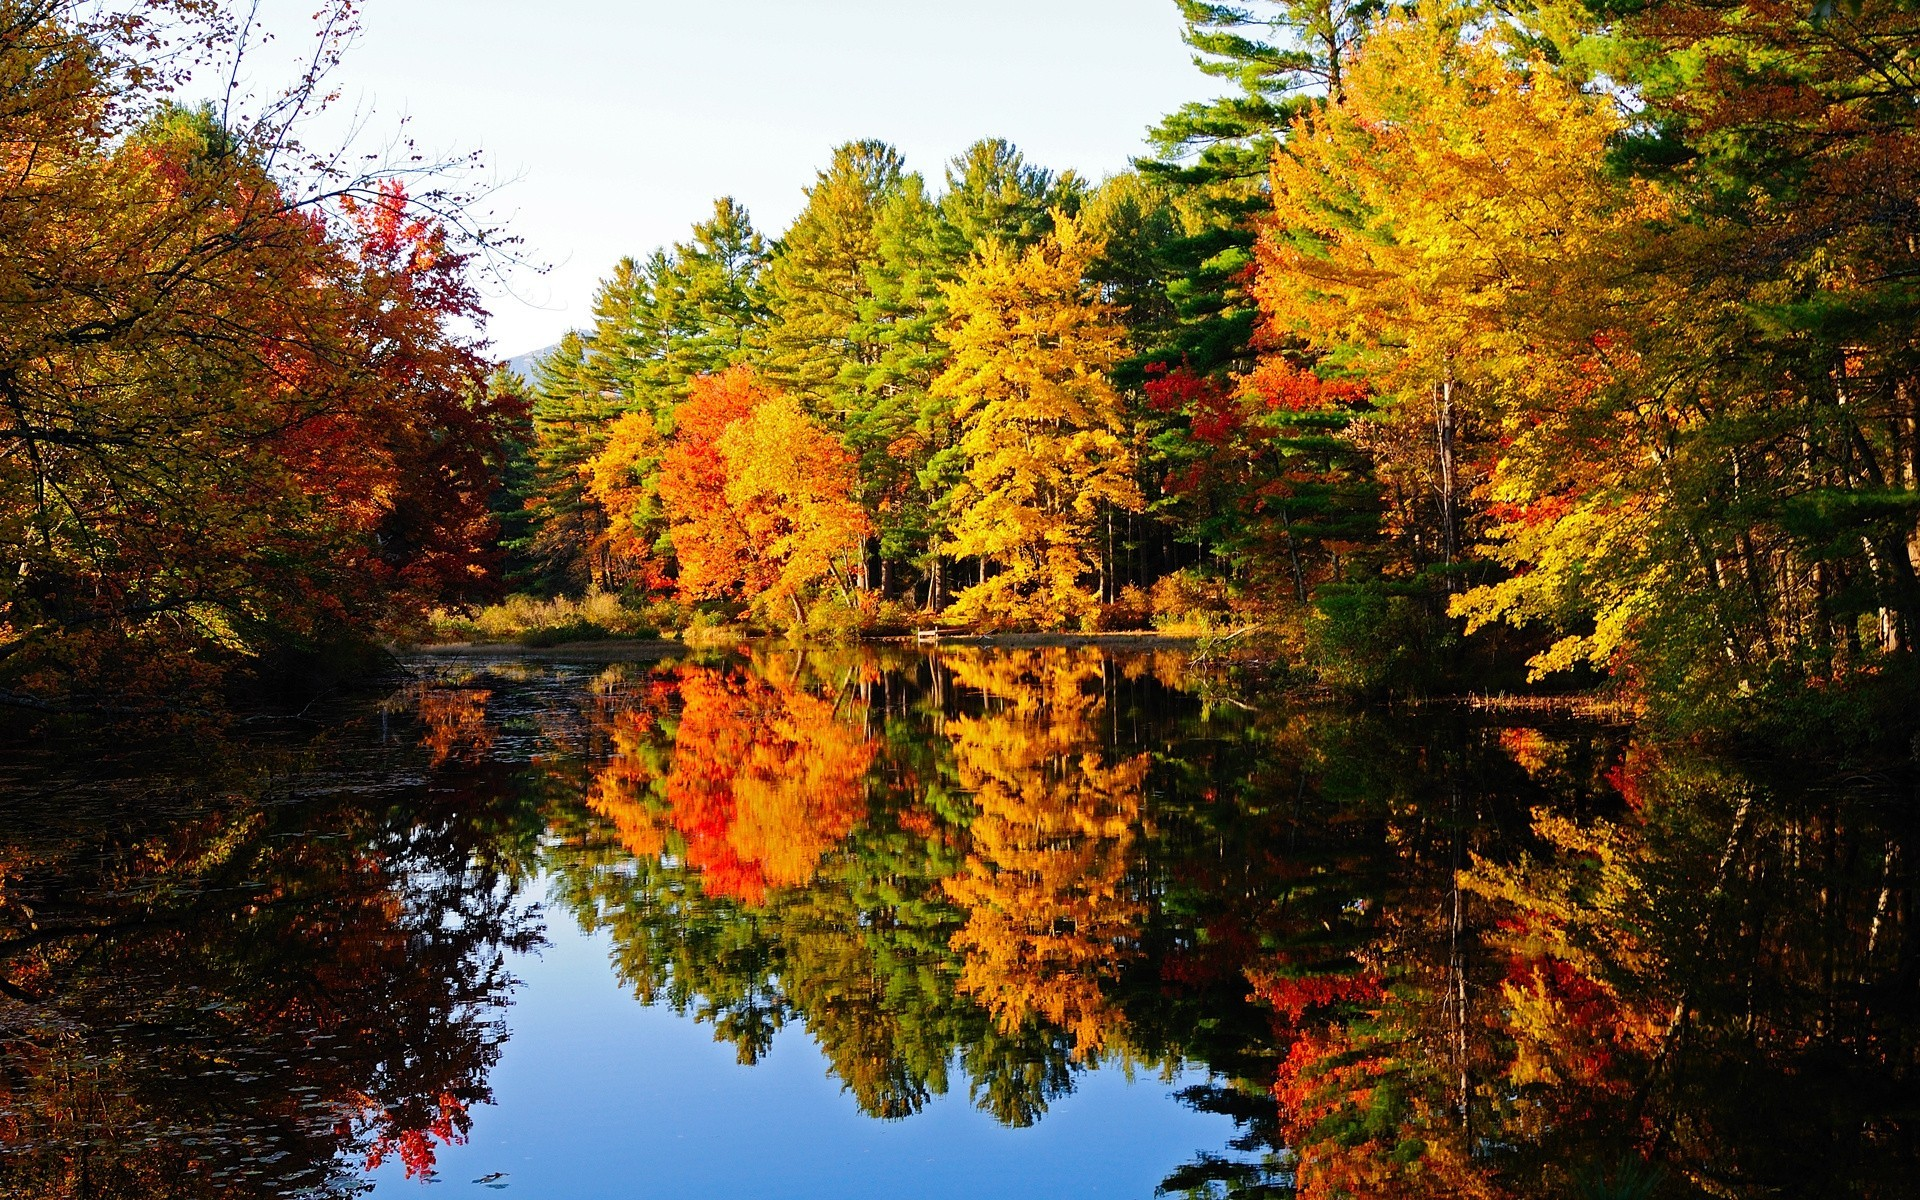
\includegraphics[width=1.0\textwidth]{image.jpg}
\caption{Осень}
\label{fig:example}
\end{figure}

\end{document}